\chapter{UAFX testing: static analysis}

The first test we conducted was the one with UAFX. Although the paper \cite{bib:uafx} explicitly states that UAFs caused by refcounts are not supported, we decided to test the tool as-is to see if it would still be able to detect the vulnerability, and then to modify it to remove the limitations imposed by the researchers and observe any changes in the results.

\section{Setup}
We started by downloading the kernel source code for version 6.6.75 from the official repository, a vulnerable version that is suitable for CVE-2025-21756 and officially supported by UAFX. To set up the environment, we installed the necessary dependencies (the most important of which include Python and LLVM version 14), \texttt{gclang}, a wrapper for the Clang compiler used to compile the source code of the relevant modules in C and generate LLVM bitcode files, and \texttt{gllvm}, a Go porting of LLVM which relies on it to extract the bitcode from the kernel source files.

UAFX also requires z3 \cite{bib:z3}, an SMT solver \cite{bib:smt} (a type of tool that checks whether a logical formula is satisfiable based on mathematical rules). It acts as a logic engine and, in our case, is used to check whether a certain path is feasible during static analysis.
\\\\
Before moving on, let's introduce some terms used in the explanation:
\begin{itemize}
    \item \textbf{bitcode}: represents the target code in LLVM Intermediate Representation (IR), the level at which UAFX performs its static analysis passes. This intermediate form is essential because it allows the tool to accurately analyze pointers and perform escape-fetch analysis, which require a code structure with more semantic information than the final binary to map the relationships between pointers even when they span multiple kernel entry functions.

    \item \textbf{object files} \texttt{(.o)}: the result of partially compiling the source code into machine code. The \texttt{.o} files are generated alongside the \texttt{.bc} files to ensure that the build environment is consistent. In our case, while the security analysis is performed on the bitcode, the original object files serve to confirm that the code is "compilable" and ready to be converted into a version that the tool can analyze.
\end{itemize}

\noindent After the initial steps, we considered two possible alternatives:
\begin{enumerate}
    \item compiling with \texttt{gllvm} \cite{bib:gllvm}/\texttt{wllvm} \cite{bib:wllvm}: these wrappers produce standard binaries and retain a reference to the bitcode, from which a single \texttt{.bc} file is then extracted;

    \item building the kernel with pure Clang/LLVM + a custom pipeline for merging \texttt{.o.bc} files.
\end{enumerate}

\noindent Since UAFX requires a single \texttt{.bc} file by default, we decided to go with the first option. \texttt{gllvm} and \texttt{wllvm} act as compiler wrappers; they generate the \texttt{.bc} files for the objects, and then \texttt{extract-bc} or \texttt{get-bc} link them into a single module, on which we can run the tool directly.

We configured some bash environment variables to ensure that LLVM and Clang use version 14:

\begin{bashlncode}
    export PATH=/usr/lib/llvm-14/bin:$PATH:$(go env GOPATH)/bin
    export LLVM_COMPILER=clang
    export LLVM_COMPILER_PATH=/usr/lib/llvm-14/bin
    export LLVM_CC_NAME=clang-14
    export LLVM_CXX_NAME=clang++-14
    export LLVM_LINK_NAME=llvm-link
    export LLVM_AR_NAME=llvm-ar-14
\end{bashlncode}

\noindent We also needed to setup the kernel source code in order to build it and extract the bitcode:

\begin{bashlncode}
    make mrproper
    make LLVM=-14 defconfig
    make LLVM=-14 menuconfig
\end{bashlncode}

\noindent These commands allow us to define which modules we're going to launch UAFX on, making the compiled kernel a valid target. Specifically:
\begin{itemize}
    \item \texttt{make mrproper} performs a complete cleanup of the kernel source tree, removing not only the object files and binaries generated by previous builds (as \texttt{make clean} would do), but also the \texttt{.config} configuration file and all automatically generated files, such as the header files produced during the build process. This ensured that we started with a completely clean source tree, eliminating any residual files that could affect the subsequent compilation. This has been particularly useful for us when running different tests with different configurations, so that we could always start from a neutral baseline.

    \item \texttt{make LLVM=-14 defconfig} generates a default kernel configuration for the current architecture, using Clang/LLVM version 14 as the compilation toolchain instead of GCC \cite{bib:gcc}. The configuration generated by \texttt{defconfig} includes a minimal set of default options, suitable for most test environments, and served as a starting point for our manual adjustments.

    \item \texttt{make LLVM=-14 menuconfig} opens an interactive menu-based interface that allows us to modify the configuration generated in the previous step. In our context, it was used to explicitly enable all components of the vsock subsystem (\texttt{VSOCK}, \texttt{VSOCK\_LOOPBACK}, \texttt{VSOCK\_DIAG}, \texttt{VMW\_VSOCK\_VIRTIO\_TRANSPORT}, and \texttt{VMW\_VSOCK\_VIRTIO\_TRANSPORT\_COMMON}), so that the compiled kernel was a suitable target for the analysis performed with UAFX.

    % TODO - immagine
\end{itemize}

\noindent Next, we have the final configuration steps and the launch of the actual build:

\begin{listing}[H]
    \bashfile{code/cmd-build.sh}
\end{listing}

\noindent With \texttt{make LLVM=-14 olddefconfig}, we reset the \texttt{.config} file to the default options for all configuration entries that were not explicitly set via \texttt{menuconfig}, because after any manual changes to the configuration, there may be unresolved symbols or unset values that could cause problems during compilation.

The following \texttt{make} command performs a series of preparatory steps that are essential for compiling external modules (in our case, UAFX). Below is a detailed explanation of the parameters:
\begin{itemize}
    \item \texttt{prepare} generates the headers and internal kernel data structures that modules need to know about at compile time, including \texttt{autoconf.h} (an auto-generated header file created during the Linux kernel build process which translates configuration options from the \texttt{.config} file into C preprocessor \texttt{\#define} macros used to compile kernel modules) and the symbol tables;

    \item \texttt{modules\_prepare} extends the preparation process to include everything needed to compile loadable modules (\texttt{.ko}), specifically the dependency files and version data for the symbols exported by the kernel (\texttt{Module.symvers});

    \item \texttt{scripts} compiles the auxiliary build tools located in \texttt{scripts/}, such as \texttt{recordmcount} and the various helper programs used by the kernel build system;

    \item \texttt{-j"\$(nproc)"} parallelizes the work across all available logical cores, speeding up the compilation steps.
\end{itemize}

\noindent Once the environment is set up, we start with the actual compilation:

%\begin{listing}[H]
%    \bashfile{code/cmd-compile.sh}
%\end{listing}

\begin{bashlncode}
make -j"$(nproc)" LLVM=-14 \
    CC=gclang HOSTCC=clang-14 HOSTCXX=clang++-14 \
    LD=ld.lld-14 AR=llvm-ar-14 NM=llvm-nm-14 \
    OBJCOPY=llvm-objcopy-14 \
    OBJDUMP=llvm-objdump-14 \
    STRIP=llvm-strip-14 \
    net/vmw_vsock/vsock.o \
    net/vmw_vsock/vmw_vsock_virtio_transport.o \
    net/vmw_vsock/vmw_vsock_virtio_transport_common.o \
    net/vmw_vsock/vsock_loopback.o \
    net/vmw_vsock/vsock_diag.o \
    net/socket.o
\end{bashlncode}

\noindent This command initiates selective compilation of only the object modules required for the analysis, explicitly specifying the entire LLVM/Clang toolchain to be used. Just as we did with the previous one, let's take a look at its structure:

\begin{itemize}
    \item \texttt{CC=gclang} replaces the C compiler with gclang, which, as we mentioned earlier, not only produces the standard object files but also generates the corresponding LLVM bitcode in parallel, which will be used by UAFX;

    \item \texttt{HOSTCC=clang-14} and \texttt{HOSTCXX=clang++-14} specify the compiler to use for build tools run on the host (such as the tools in \texttt{scripts/}), which is different from the target compiler;

    \item \texttt{LD}, \texttt{AR}, \texttt{NM}, \texttt{OBJCOPY}, \texttt{OBJDUMP}, and \texttt{STRIP} replace the corresponding \texttt{binutils} tools (used in the compilation process) with their LLVM counterparts.
\end{itemize}

\noindent After the \texttt{STRIP} parameter, we have a set of targets that correspond to the vsock subsystem modules selected during the \texttt{menuconfig} phase, plus \texttt{net/socket.o}, which implements the generic socket interface at the kernel level and is required to resolve symbol dependencies. The result is a set of \texttt{.o} files, from which we extract the bitcode:

\begin{bashlncode}
get-bc -o 
    ../uafx/_bc/vsock.bc
    net/vmw_vsock/vsock.o
get-bc -o
    ../uafx/_bc/vmw_vsock_virtio_transport.bc
    net/vmw_vsock/vmw_vsock_virtio_transport.o
get-bc -o
    ../uafx/_bc/vmw_vsock_virtio_transport_common.bc
    net/vmw_vsock/vmw_vsock_virtio_transport_common.o
get-bc -o
    ../uafx/_bc/vsock_loopback.bc
    net/vmw_vsock/vsock_loopback.o
get-bc -o
    ../uafx/_bc/vsock_diag.bc
    net/vmw_vsock/vsock_diag.o
get-bc -o
    ../uafx/_bc/socket.bc
    net/socket.o
\end{bashlncode}

\noindent Here we use \texttt{get-bc}, a utility from the wllvm toolkit (on which gllvm is based), which retrieves the LLVM bitcode previously embedded by gclang within each \texttt{.o} object file and exports it to standalone \texttt{.bc} files. As mentioned, LLVM bitcode is an intermediate representation of the source code, independent of the target architecture, that preserves high-level semantic information that would otherwise be lost in traditional compilation to machine code. The elements of interest to us, for use with UAFX, are the types, the call graph, and the relationships between instructions (which are extremely important for escape-fetch-based cross-entry alias analysis, specifically in the reconstruction of object paths). The \texttt{socket.bc} file is included to allow UAFX to resolve the symbols in the kernel's generic socket layer that the vsock modules reference.

As the final step in the general configuration, we set up the list of functions to be considered as entry points by UAFX, a partial list of which is provided below:
\begin{bashlncode}
vsock_create
vsock_bind
vsock_remove_sock
...
__sys_socket
__sys_bind
__sys_connect
...
\end{bashlncode}
It is important to note that some of the functions we have included are defined within the Linux kernel as \textbf{syscalls} (system calls) \cite{bib:syscalls}. They constitute the interface through which user-space programs request services from the kernel (e.g. creating a socket, establishing a connection) passing through syscall-specific macros, which generate the architecture-dependent entry points and the intermediate wrappers required to dispatch a request to its actual implementation. For example, a user-space operation like \texttt{connect()} traces back to kernel functions such as \texttt{\_\_sys\_connect()}, before being dispatched to the protocol-specific implementation through the socket operation interface.

This presented another potential obstacle because the UAFX paper does not mention any support for functions of this type, nor does it explicitly rule them out. Since the objects we are considering necessarily go through these functions as well, we had to add them to the set of entry functions for UAFX.

\noindent At this point, we had two options:
\begin{enumerate}
    \item include them directly as separate modules (even though the paths between modules would remain incomplete);
    
    \item link the modules and run UAFX on a cumulative bitcode.
\end{enumerate}
The first option involved running UAFX on the modules separately. In this case, only UAFs related to issues within individual modules would have been detected (and thus much less likely to have gone undetected than a UAF affecting multiple modules). With this approach, the configuration ends here.

The second method, on the other hand, requires a few additional configuration steps. As mentioned earlier, the goal was to combine all the modules in question into a single cumulative module so that it could be fed to UAFX all at once, taking into account all the functions of all the modules.

\clearpage
\noindent As a first step in this process, we had to disassemble some of the modules:

\begin{bashlncode}
llvm-dis-14 
    vsock_loopback.bc
    -o /tmp/vsock_loopback.ll
llvm-dis-14
    vsock_diag.bc
    -o /tmp/vsock_diag.ll
llvm-dis-14
    vmw_vsock_virtio_transport.bc
    -o /tmp/virtio_transport.ll
llvm-dis-14
    vmw_vsock_virtio_transport_common.bc
    -o /tmp/virtio_common.ll
\end{bashlncode}

\noindent We had to do this to rename certain definitions that were repeated across modules. Specifically, the functions \texttt{init\_module} and \texttt{cleanup\_module} are defined in multiple modules among those we chose to merge. When considered as individual modules, they pose no problem, but once combined, they trigger an error due to the multiple definition of symbols. Since the names of the functions within the individual modules are arbitrary, we simply renamed them to make them unique. We provide just one example of the command used to do this, but the renamed functions are located in the modules \texttt{vsock\_loopback}, \texttt{vsock\_diag}, \texttt{virtio\_transport}, and \texttt{virtio\_common}.

\begin{bashlncode}
sed -i \
  -e 's/@init_module/@init_module_vsock_loopback/g' \
  -e 's/@cleanup_module/@cleanup_module_vsock_loopback/g' \
  /tmp/vsock_loopback.ll
...
\end{bashlncode}

\noindent After the modification, we reassemble the impacted modules to regenerate the bitcode:

\begin{bashlncode}
llvm-as-14
    /tmp/vsock_loopback.ll
    -o vsock_loopback_renamed.bc
llvm-as-14
    /tmp/vsock_diag.ll
    -o vsock_diag_renamed.bc
llvm-as-14
    /tmp/virtio_transport.ll
    -o vmw_vsock_virtio_transport_renamed.bc
llvm-as-14
    /tmp/virtio_common.ll
    -o vmw_vsock_virtio_transport_common_renamed.bc
\end{bashlncode}

\noindent After that, we can proceed to link the modules to create a combined module, on which UAFX will be launched.

\begin{bashlncode}
llvm-link \
    vsock.bc \
    vsock_loopback_renamed.bc \
    vsock_diag_renamed.bc \
    vmw_vsock_virtio_transport_renamed.bc \
    vmw_vsock_virtio_transport_common_renamed.bc \
    socket.bc \
    -o _vsock_all.bc
\end{bashlncode}

\section{Test execution}

The UAFX testing phase was conducted in two stages. As explained earlier, the UAFX paper explicitly states that reference counting issues have been ruled out. The first phase consisted of testing directly using the unmodified version of UAFX. In the second phase, we modified the UAFX code to remove the constraints that rule out reference counting issues and repeated the tests on the same target bitcode.

\subsection{Test with unmodified UAFX}
As mentioned, the first test was conducted using UAFX as provided by the researchers, with controls in place to rule out active reference counting issues. We ran the script provided by the researchers on the unified bitcode:

\begin{bashlncode}
./run_nohup.sh _bc/_vsock_all.bc results/_conf_uafx_vsock
\end{bashlncode}

\noindent Figure \ref{fig:uafx-execution-unmodified} represents an example of the output from running UAFX on the extracted bitcode.

\begin{figure}[h]
    \centering
    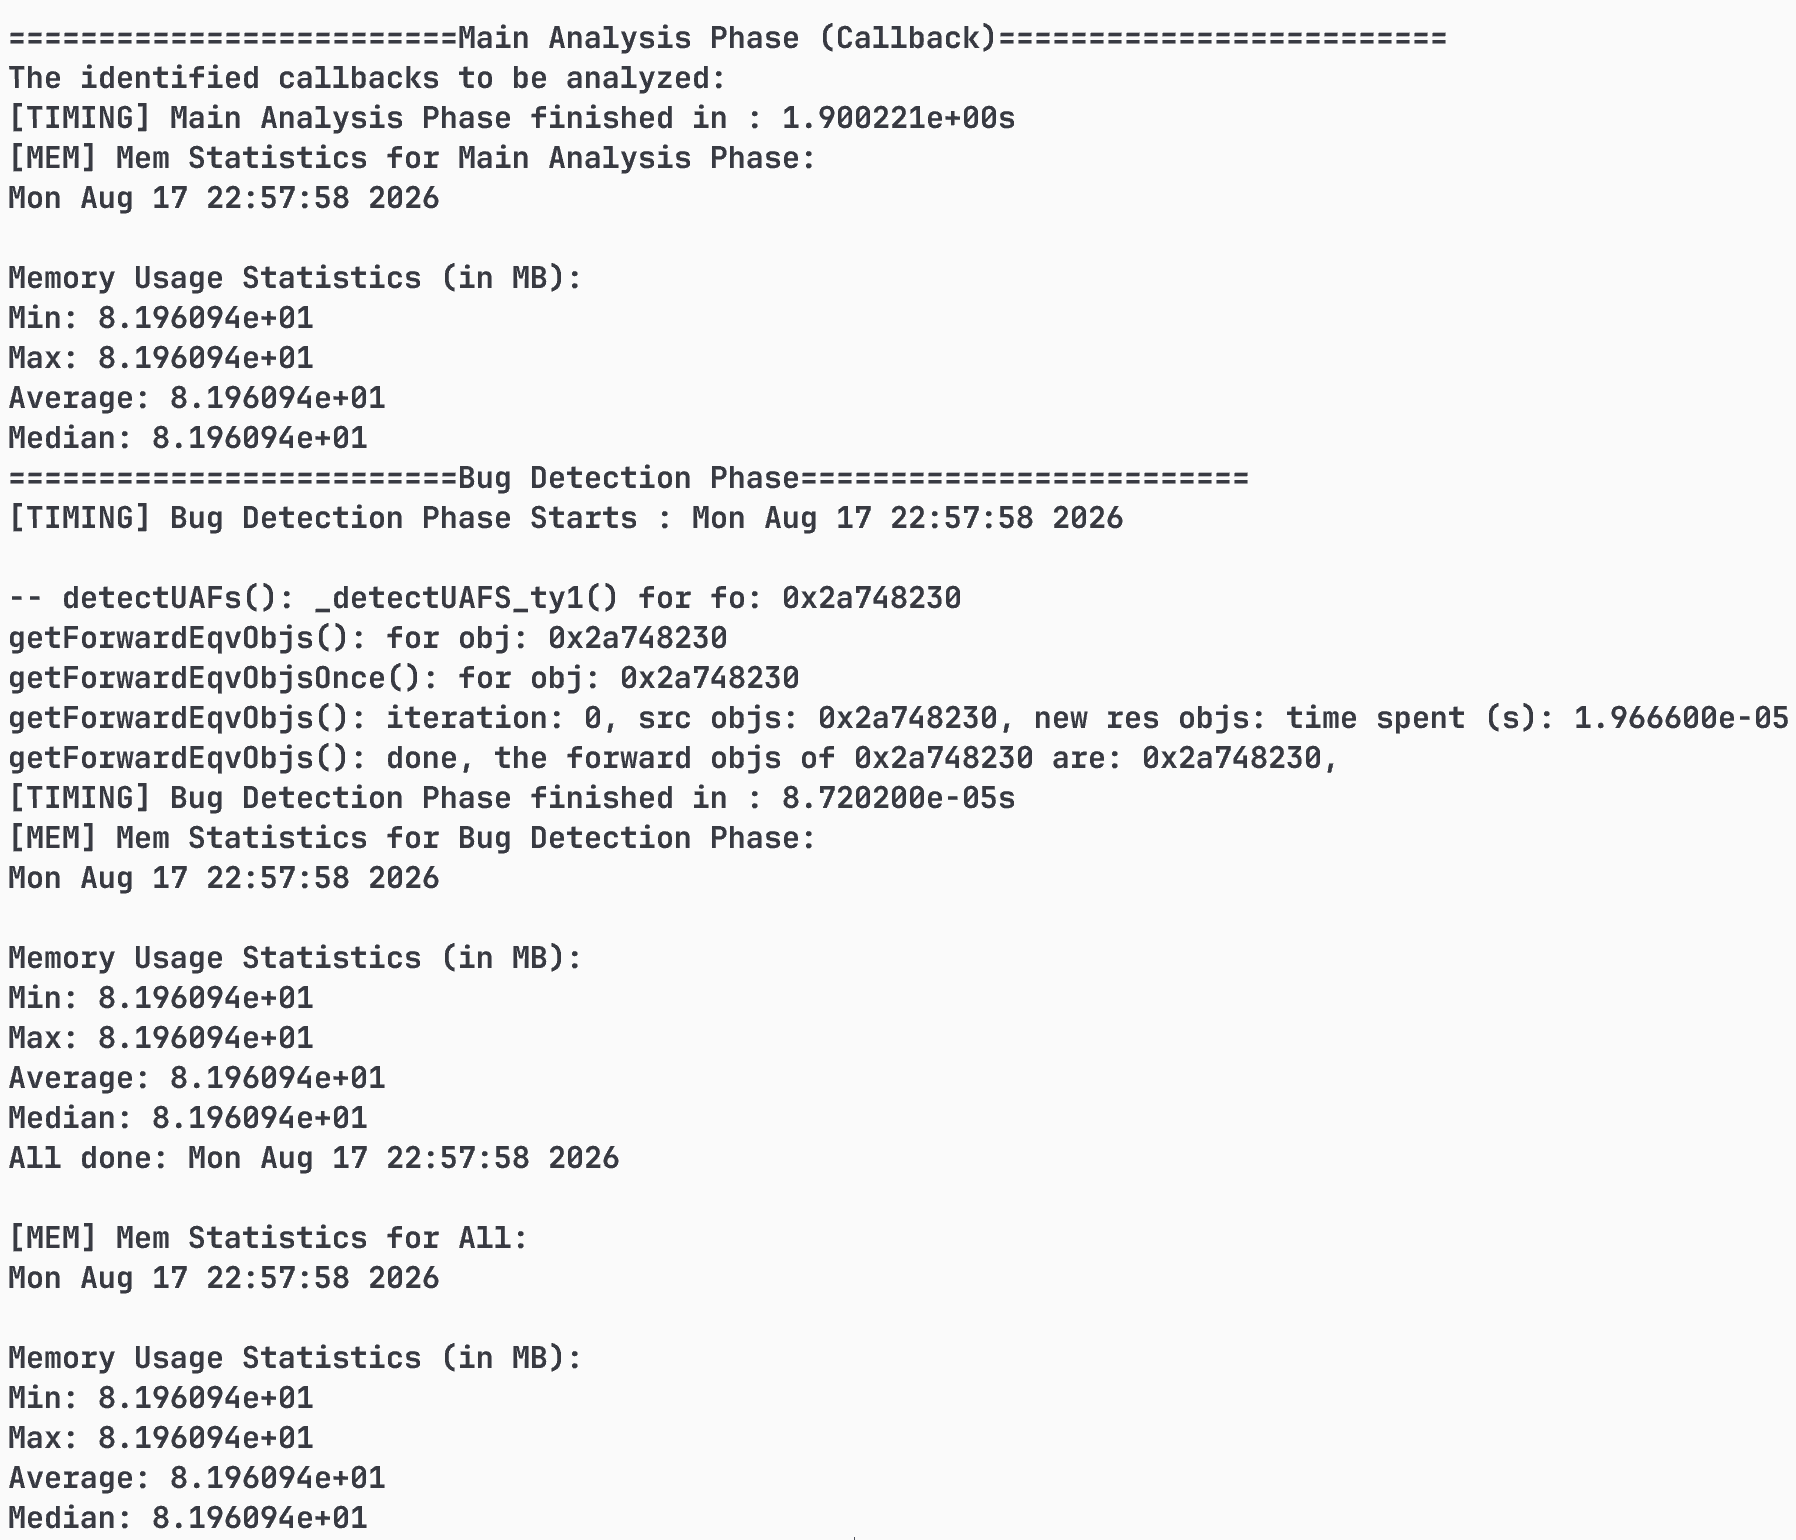
\includegraphics[scale=.67]{images/uafx-execution-unmodified.png}
    \caption{Execution results with unmodified UAFX.}
    \label{fig:uafx-execution-unmodified}
\end{figure}

\noindent As we can see, running UAFX on the aggregated bitcode completes successfully, finishing both the Main Analysis Phase and the subsequent \textit{Bug Detection }Phase, but the analysis does not produce any reports of potential use-after-free vulnerabilities.

Specifically, during the phase dedicated to callback analysis, the section titled "\textit{The identified callbacks to be analyzed}" is empty, so UAFX hasn't identified any additional callbacks to be subjected to the interprocedural analysis.

During the Bug Detection Phase, a candidate object \texttt{(fo)} is considered, on which the \texttt{\_detectUAFS\_ty1()} procedure is executed. UAFX then attempts to determine its equivalent objects using \texttt{getForwardEqvObjs()}, but the propagation reaches a dead end as early as the first iteration: the resulting set contains only the starting object, and no additional equivalent objects are identified to which the analysis can be propagated.

Consequently, in this configuration, UAFX is unable to establish a connection between the candidate under consideration and a subsequent access that could be classified as a use-after-free. We can in fact see that the Bug Detection Phase ends in an extremely short amount of time (approximately $8.7 \times 10^{-5}$ seconds) without generating any warnings.

This result does not prove the absence of the vulnerability in the analyzed code, but it indicates that, with the provided bitcode, entry functions, and using the standard UAFX configuration, the analysis failed to reconstruct a flow sufficient to trigger the UAF under investigation. We can assume that this could be caused by insufficient interprocedural propagation or the failure to resolve callbacks or indirect calls involved in the vulnerable path. Another possible cause could have been the explicitly mentioned exclusion of reference counting issues, for which we made a change to UAFX, as described below.

\subsection{Test with modified UAFX}

To modify UAFX, we traced the code execution flow starting from the entry point. Reference counting issues are filtered in \texttt{ModuleState.h} by calling the \texttt{\_isWithRefcnt} function defined in \texttt{ModuleState.cpp} as follows: 

\begin{listing}[H]
    \cfile{code/isWithRefcnt.c}
\end{listing}

\noindent The function implements a lightweight heuristic to recognize cases in which a potential UAF is likely protected by a reference counting mechanism. It receives the free location and the use location, but in the current implementation it mainly reasons about the free site.

The first heuristic checks whether the free operation occurs inside, or through, a function whose name suggests a reference-count decrement/release operation. In particular, the analysis collects the instruction corresponding to the free site and the call sites in its calling context, then walks this sequence backwards and inspects the name of each enclosing function. If one of these function names contains patterns such as \texttt{\_put} or \texttt{put\_} (lines 4-7), the function assumes that the free may be guarded by a reference counting \texttt{put} operation and returns \texttt{true}.

The same check is also applied to function names recovered from debug information, which is useful because debug metadata can expose inlined function names that are not directly visible from the LLVM instruction's enclosing function and the heuristic can also detect cases where the reference-counting operation was inlined.

The function also defines patterns for reference-count acquisition functions, such as \texttt{\_get} and \texttt{get\_} (lines 8-11), but these are not effectively used by the current heuristic.

At line 51, we omitted some comments from the original code \cite{bib:uafx-code} that mention possible future development of two additional heuristics:
\begin{itemize}
    \item \textbf{Heuristic 2}: check whether the free site is dominated or post-dominated by an update to the reference count;

    \item \textbf{Heuristic 3}: check whether the usage site is protected by a change in the reference count.
\end{itemize}
At the time of writing, these heuristics have not yet been implemented, and therefore we have not taken them into account.

Overall, this is just a syntactic filter: it doesn't model the actual value of the reference counter, but instead it treats the presence of a likely reference-count release function in the free-side context as evidence that the reported UAF may be a false positive caused by imprecise reasoning about reference counting.

After making the change by disabling the check, we recompiled UAFX and relaunched it using the same bitcode as the execution with the checks enabled. However, the results are no different from the previous ones, as we can see in figure \ref{fig:uafx-execution-modified}.

\begin{figure}[h]
    \centering
    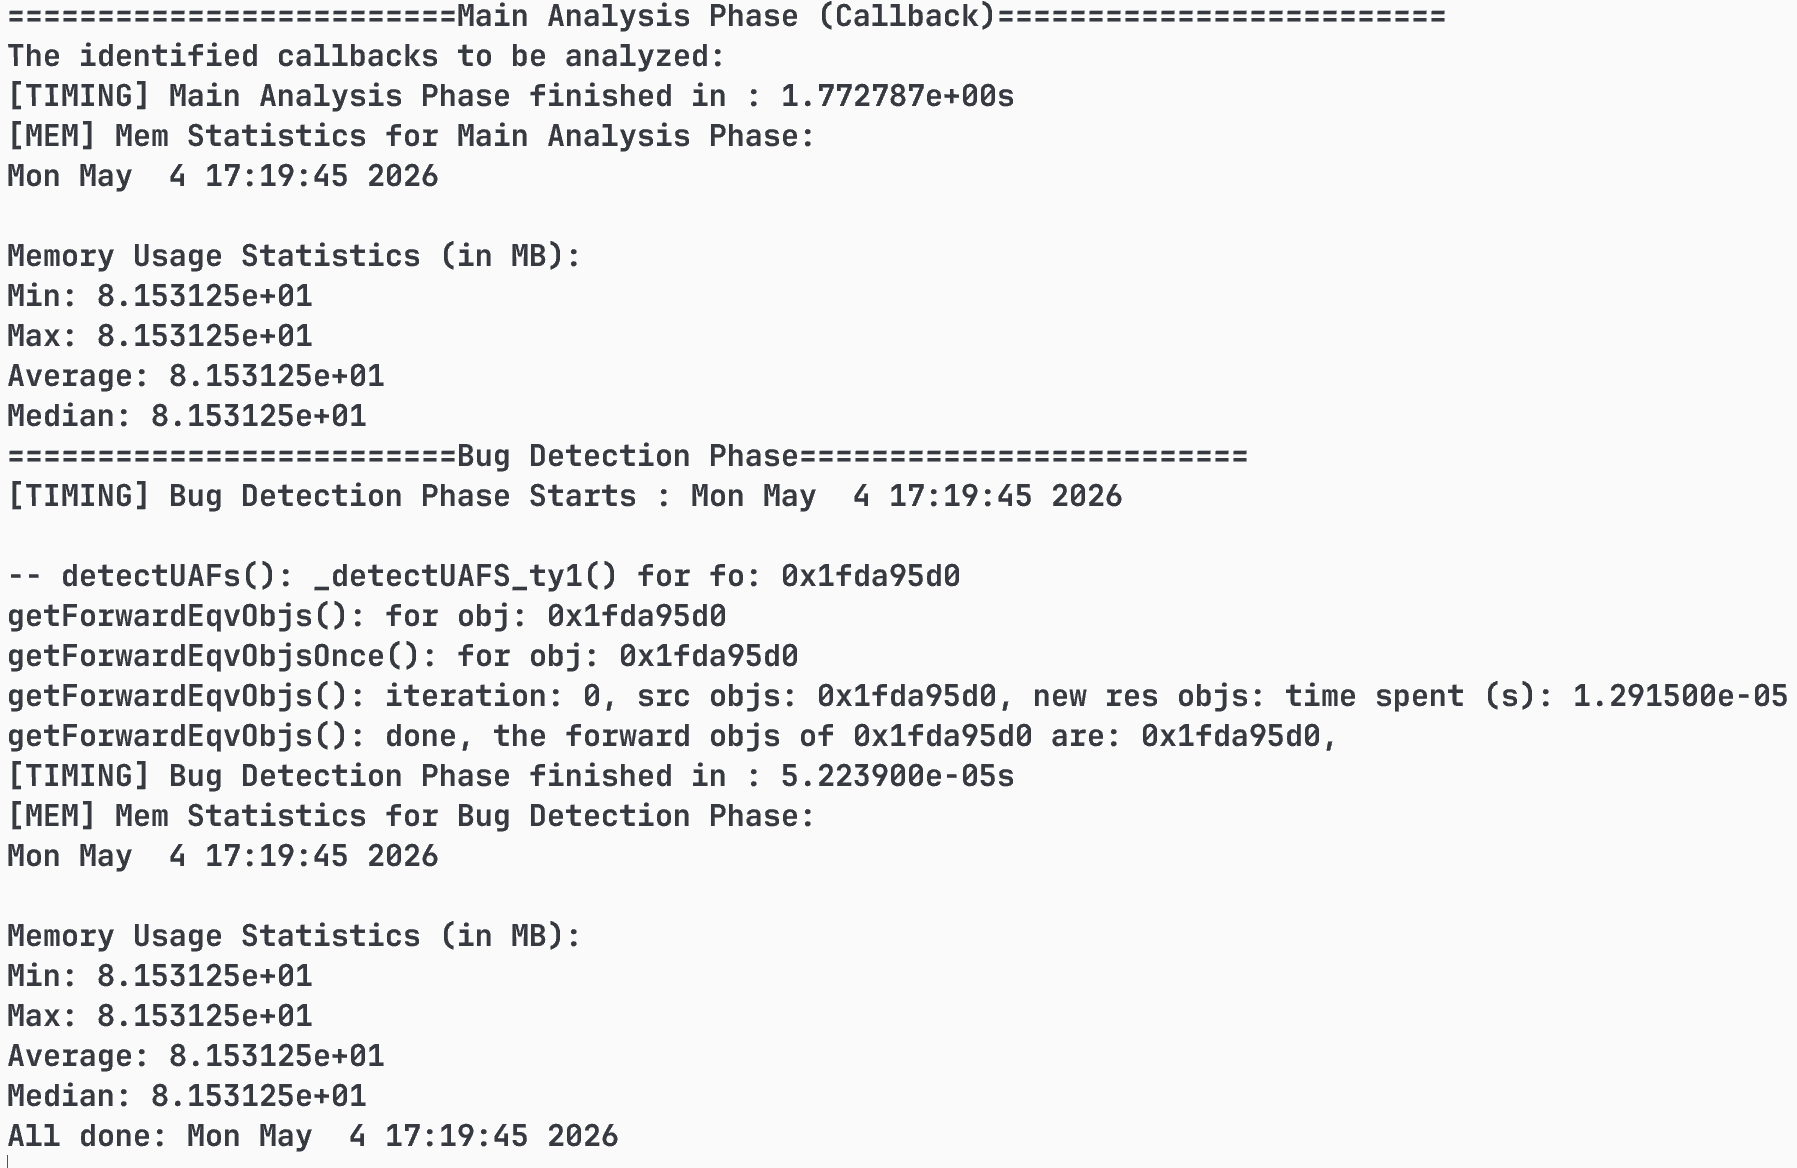
\includegraphics[scale=.22]{images/uafx-execution-modified.png}
    \caption{Execution results with modified UAFX.}
    \label{fig:uafx-execution-modified}
\end{figure}

\noindent In this case as well, no callbacks are identified for analysis and, during the \textit{Bug Detection Phase}, a single candidate object is considered. The search for equivalent objects in the forward direction immediately reaches a dead end, leaving only the initial object and failing to identify any further relationships useful for constructing a possible UAF path.

Removing the filter related to reference counting is therefore not sufficient, in this case, to reveal the vulnerability. This comparison also allows us to put into perspective the hypothesis formulated following the first execution: the absence of warnings does not appear to be caused solely by the intentional exclusion of reference counting cases, since the behavior of the analysis remains virtually unchanged even without that filter.

The limitation appears to arise at an earlier or different stage of the analysis, for example in the identification and propagation of relationships between objects, or in the reconstruction of the interprocedural flow required to link the creation of an object to its subsequent use. These results, however, don't allow us to determine which of these mechanisms is responsible for the failure to detect the issue.